%**************************************************************************************
% License:
% CC BY-NC-SA 4.0 (http://creativecommons.org/licenses/by-nc-sa/4.0/)
%**************************************************************************************

\documentclass[notes]{beamer}

\mode<presentation> {

\usetheme{Madrid}

% Burnt orange
\definecolor{burntorange}{rgb}{0.8, 0.33, 0.0}
\colorlet{beamer@blendedblue}{burntorange}
% Pale yellow
\definecolor{paleyellow}{rgb}{1.0, 1.0, 0.953}
\setbeamercolor{background canvas}{bg=paleyellow}
% Secondary and tertiary palett
\setbeamercolor*{palette secondary}{use=structure,fg=white,bg=burntorange!80!black}
\setbeamercolor*{palette tertiary}{use=structure,fg=white,bg=burntorange!60!black}

% To remove the footer line in all slides uncomment this line
%\setbeamertemplate{footline}
% To replace the footer line in all slides with a simple slide count uncomment this line
%\setbeamertemplate{footline}[page number]

% To remove the navigation symbols from the bottom of all slides uncomment this line
%\setbeamertemplate{navigation symbols}{}
}

\usepackage{amsmath}
\usepackage{bm}
\usepackage{breqn}
\usepackage{graphicx} % for figures
\usepackage{subcaption} % for subplots 
\usepackage[labelsep=space,tableposition=top]{caption}
\renewcommand{\figurename}{Fig.} 
\usepackage{cleveref}
\usepackage{caption,subcaption}% http://ctan.org/pkg/{caption,subcaption}
\usepackage{booktabs} % Allows the use of \toprule, \midrule and \bottomrule in tables
\usepackage{multirow}

% To print 2 slides on a page
%\usepackage{handoutWithNotes}
%\pgfpagesuselayout{2 on 1}[border shrink=2mm]
%----------------------------------------------------------------------------------------
%	TITLE PAGE
%----------------------------------------------------------------------------------------
% The short title appears at the bottom of every slide, the full title is only on the title page
\title[CE394M: solvers - errors]{CE394M: FEM solvers and errors} 
\author{Krishna Kumar} % name
\institute[UT Austin] % institution 
{
University of Texas at Austin \\
\medskip
\textit{
  \url{krishnak@utexas.edu}} % Your email address
}
\date{\today} % Date, can be changed to a custom date

\begin{document}

\begin{frame}
\titlepage % title page as the first slide
\end{frame}

\begin{frame}
 % Table of contents slide, comment this block out to remove it
 \frametitle{Overview}
 % Throughout your presentation, if you choose to use \section{} and \subsection{} 
 % commands, these %will automatically be printed on this slide as an overview 
 \tableofcontents
\end{frame}

%----------------------------------------------------------------------------------------
% slides
%----------------------------------------------------------------------------------------
\section{Solving non-linear problems}
%------------------------------------------------
\begin{frame}
\frametitle{Linear and non-linear problems}
\begin{itemize}
	\item \textbf{Linear problems}
	\mode<beamer>{
		\begin{itemize}
			\item The response can only be approximated as linear if its
			deformations/motions are small.
			\item In linear analyses, the response to individual load cases can be
			scaled and added to the results from other linear analyses,
			which is the principle of superposition.
		\end{itemize}
	}
	\mode<handout>{
		\vspace{2.5cm}
	}
	%
	\item \textbf{Non-linear problems}
		\mode<beamer>{
		\begin{itemize}
			\item Superposition is invalid.
			\item The solution is an incremental/iterative process.
			\item An iteration is the solution of a system of equations linearised
			about the current state of the nonlinear physical problem.
		\end{itemize}
	}
	\mode<handout>{
		\vspace{2.5cm}
	}
	\end{itemize}
\end{frame}

%------------------------------------------------
\begin{frame}
\frametitle{Non-linearity in geotechnical engineering}
\mode<beamer>{
	\begin{itemize}
		\item \textbf{Material non-linearity}
			\begin{itemize}
				\item plasticity
			\end{itemize}

		\item \textbf{Contact}
			\begin{itemize}
				\item discontinuous source of non-linearity
			\end{itemize}
		
		\item \textbf{Large deformations and motions of a geotechnical structures}
			\begin{itemize}
				\item rotation, rigid body motion
				\item often ignored, still in the research area.
			\end{itemize}
	\end{itemize}
}
\mode<handout>{
	\vspace{3cm}
}
	%
\begin{figure}[ht]
	\centering
	
\includegraphics[width=0.85\textwidth]{figs/rotation.png}
	\caption*{No strains if linear strain-displacement relations are used.}
\end{figure}
\end{frame}

%------------------------------------------------
\begin{frame}
\frametitle{Linear solvers}
To solve a system of linear equations of the form $\mathbf{Ka = b}$, there are two families of
methods of solvers that can be used: direct and iterative.
\mode<beamer>{
	\begin{itemize}
		\item Direct solvers solve a system of linear equations in a predefined number of steps. 
		\item Methods are based on Gauss elimination, with the most common method being LU decomposition. 
		\item The time required to solve a linear system increases with the number of computer
		operations performed.
		\item For a direct linear solver applied to a dense system of size $n \times n$: CPU time = $C n^3$.
		\item If the number of degrees of freedom in a finite element simulation is doubled,
		the time required to solve the system will increase by a factor of 8!
	\end{itemize}
}
\mode<handout>{
	\vspace{6cm}
}
\end{frame}

\subsection{Tangent stiffness}
%------------------------------------------------
\begin{frame}
\frametitle{Tangent stiffness method}
\mode<beamer>{
	\begin{figure}[ht]
		\centering
		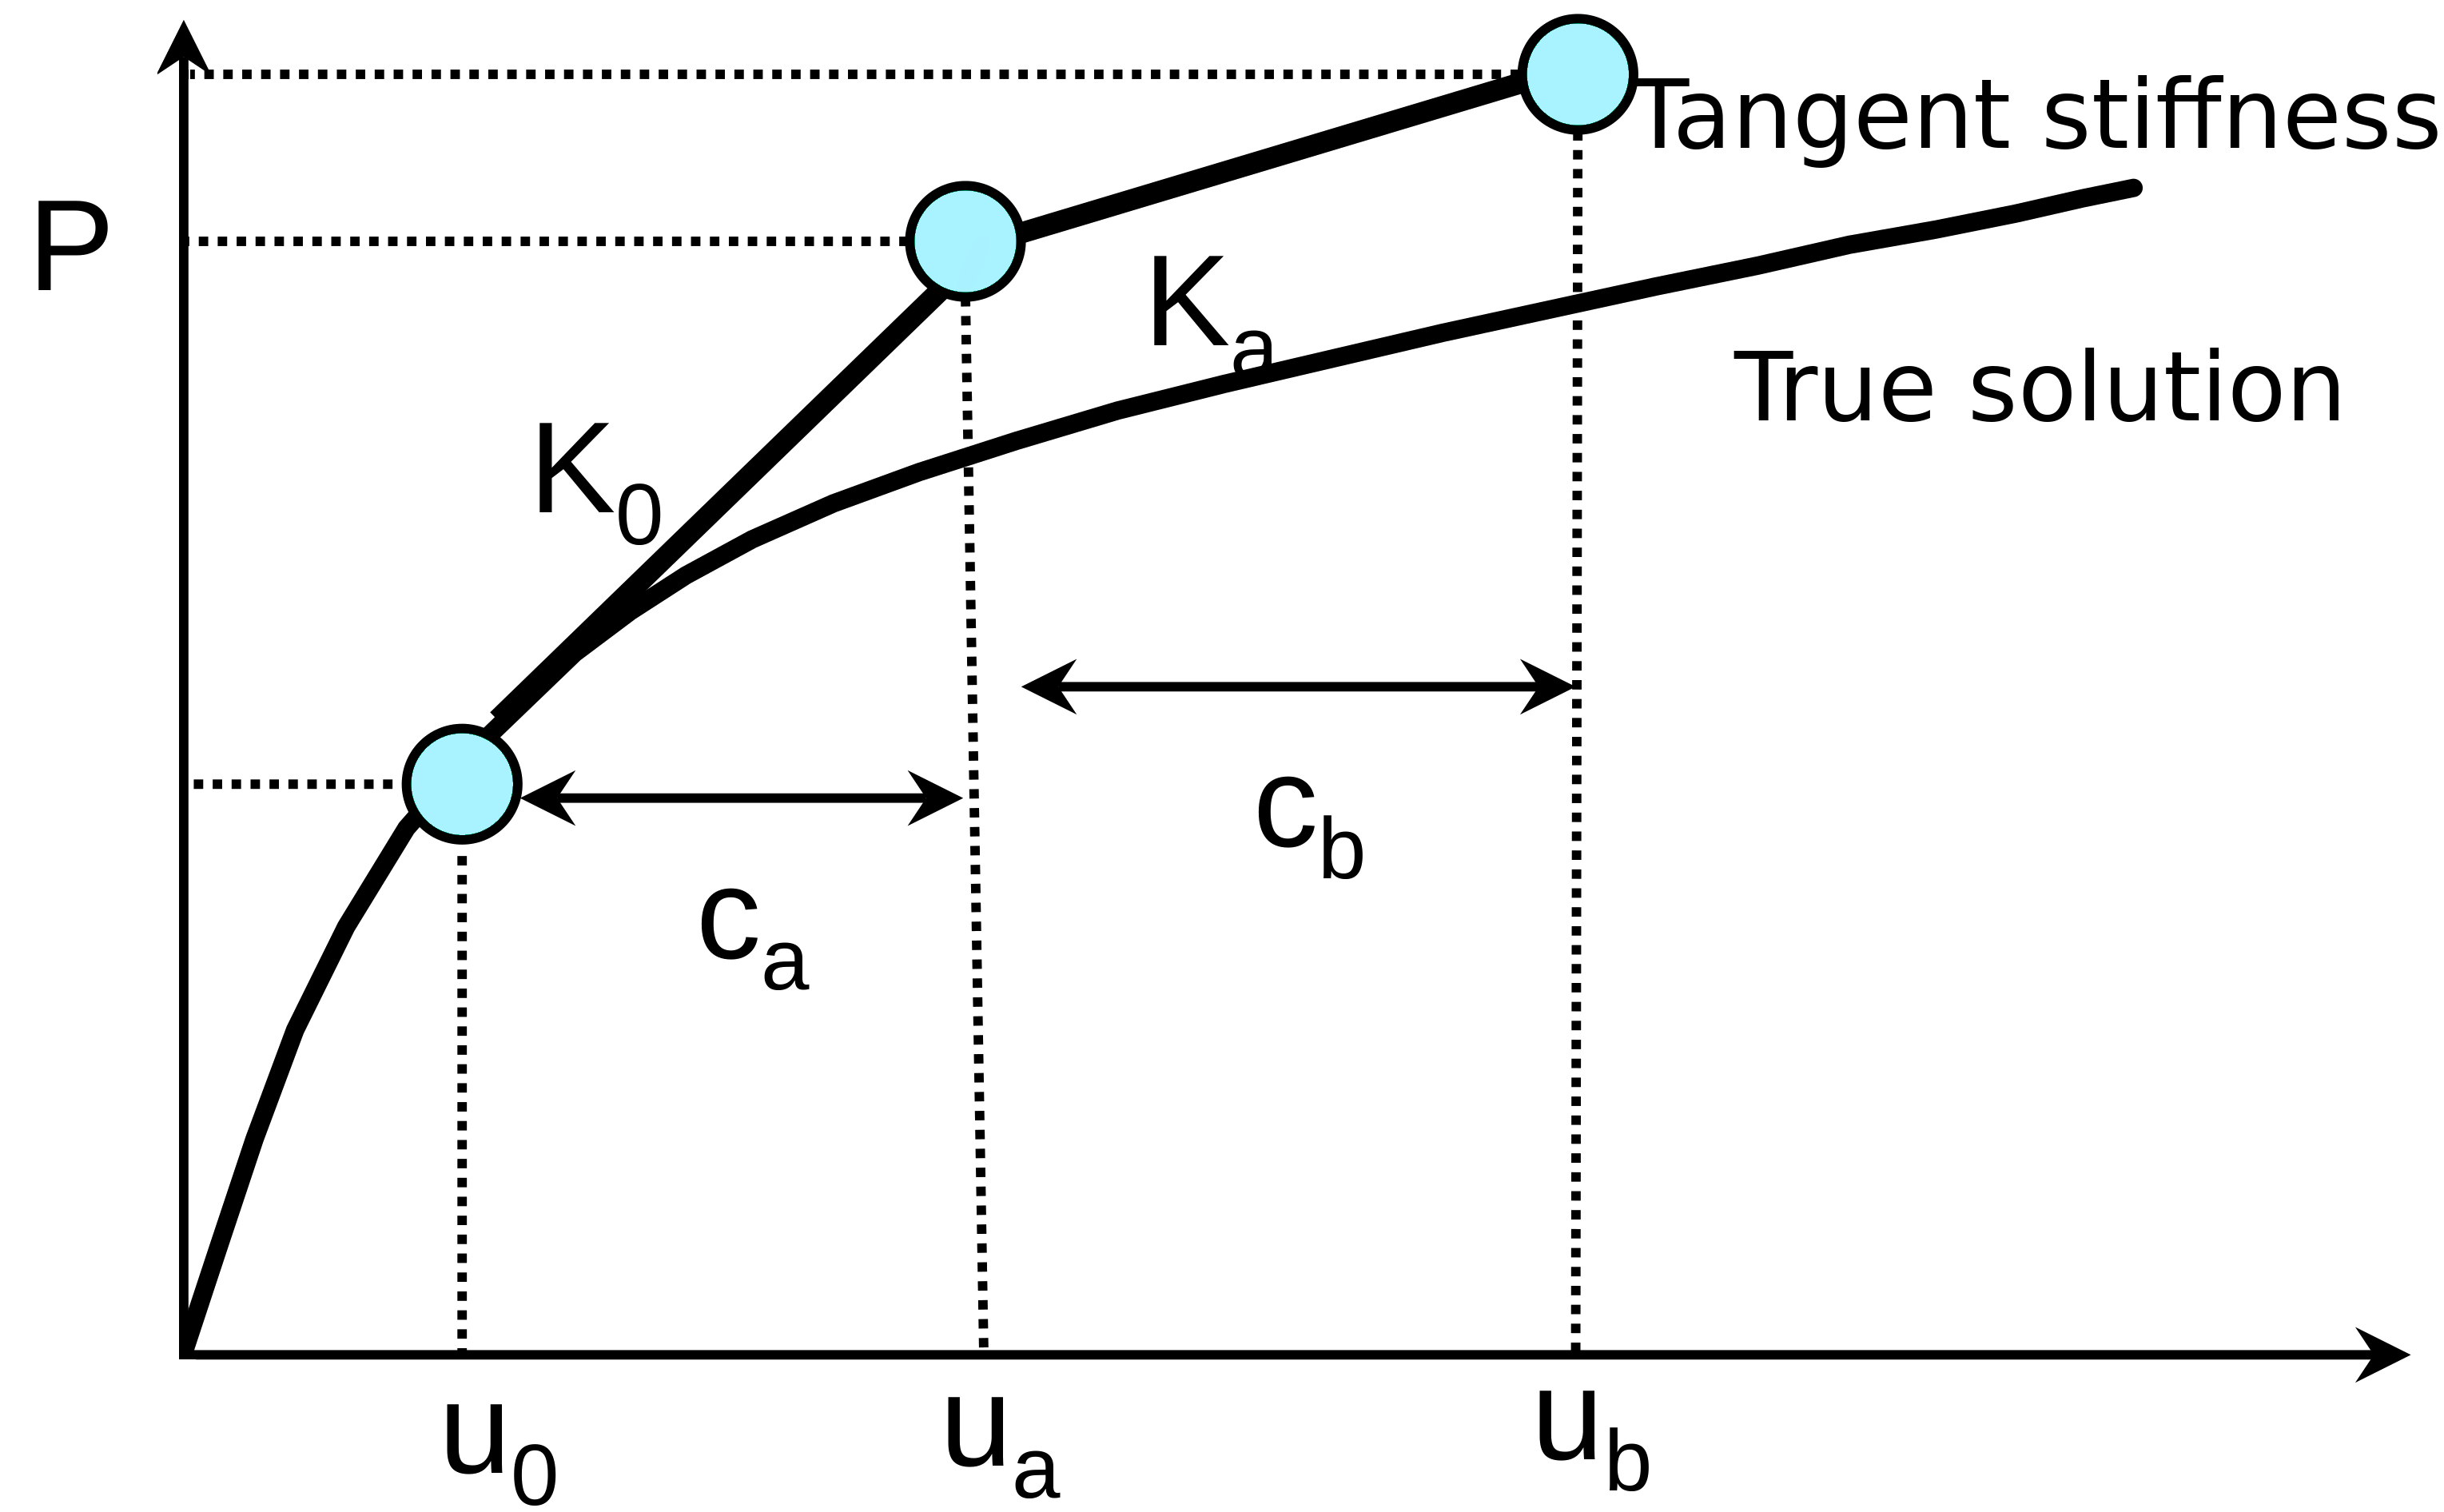
\includegraphics[width=0.65\textwidth]{figs/tangent-stiffness.png}
	\end{figure}
	\begin{itemize}
		\item Many small increments are need to obtain accurate solution
		\item Need to perform a parametric study to find the optimum incremental
		\item Defining increments is very important
		\item Program - SAGE CRISP
	\end{itemize}
}
\mode<handout>{
	\vspace{6cm}
}
\end{frame}
\note{
	In the incremental solution we divide the load into increments $\Delta P = \lambda P$, where $\lambda$ is also known as a load factor and apply a repeated solution of $\Delta u = K^{-1} \Delta P$. \\
	
	Basically we divide the load into substeps, and treat each as linear - but that is usually not accurate enough and inefficient.
}
\subsection{Newton Raphson}
%------------------------------------------------
\begin{frame}
\frametitle{Newton Raphson method}
\mode<beamer>{
	\begin{figure}[ht]
		\centering
		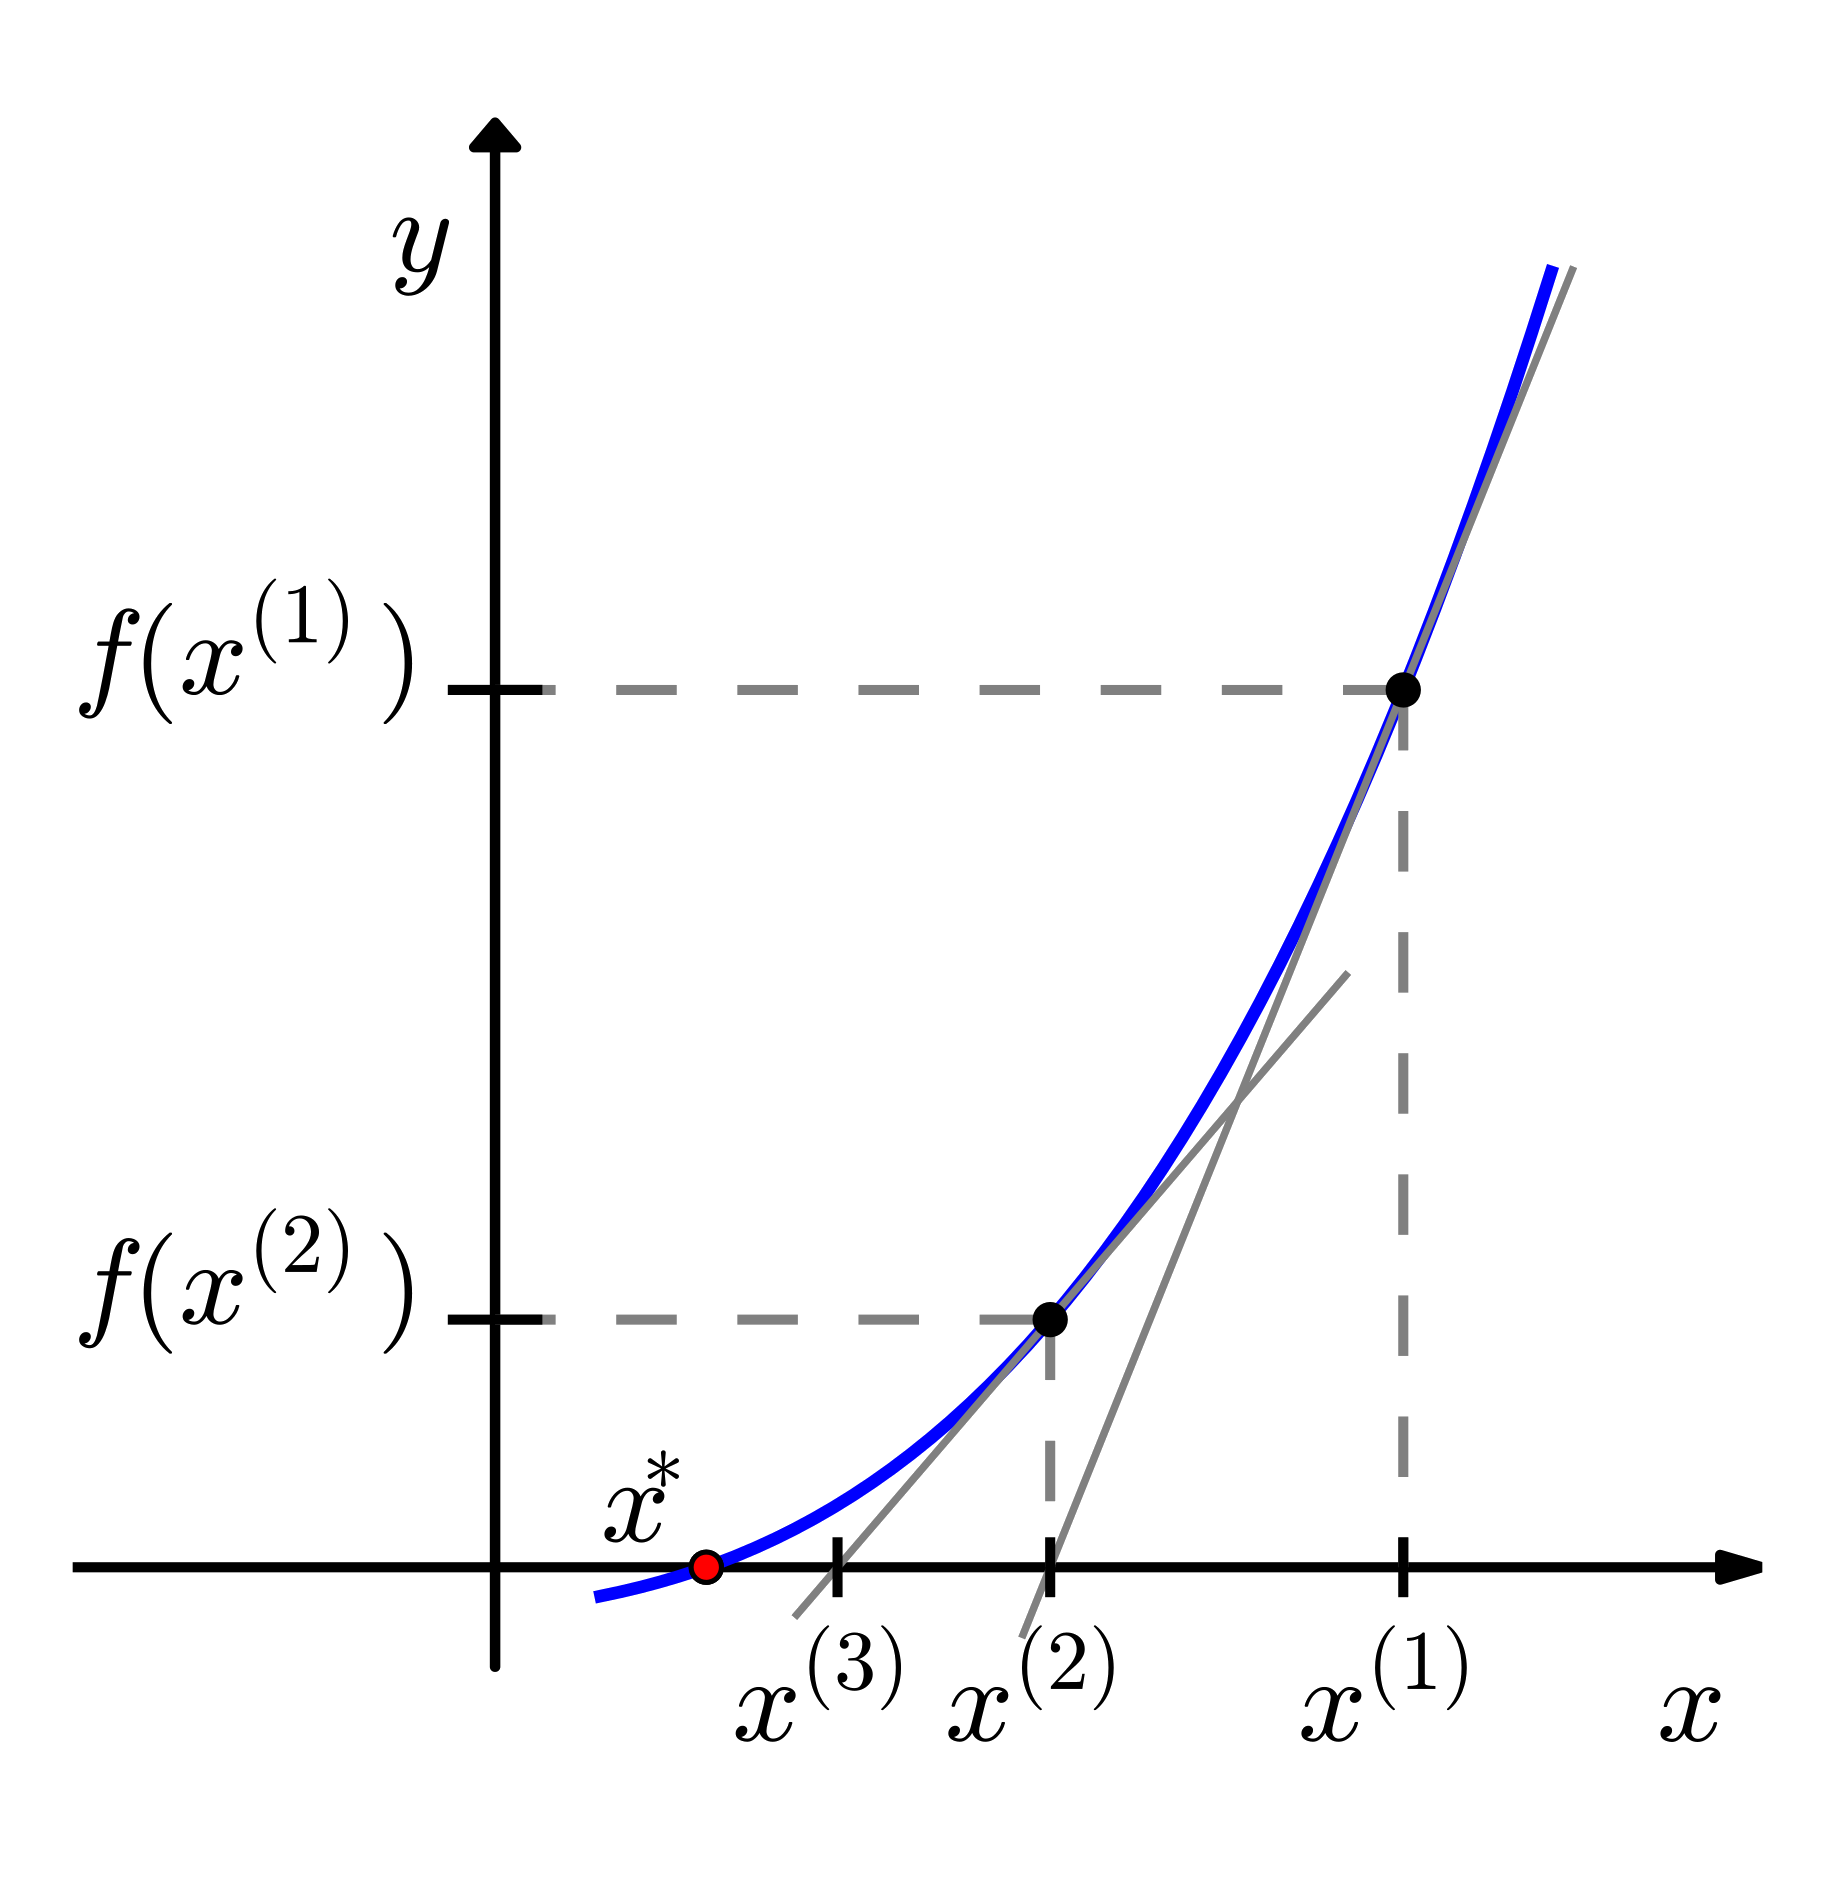
\includegraphics[width=0.5\textwidth]{figs/newton.png}
	\end{figure}
	\begin{equation*}
		x_{n+1} = x_n - \frac{f(x_n)}{f^\prime(x_n)}
	\end{equation*}
}
\mode<handout>{
	\vspace{6cm}
}
\end{frame}

%------------------------------------------------
\begin{frame}
\frametitle{Newton Raphson method}
\mode<beamer>{
	\begin{figure}[ht]
		\centering
		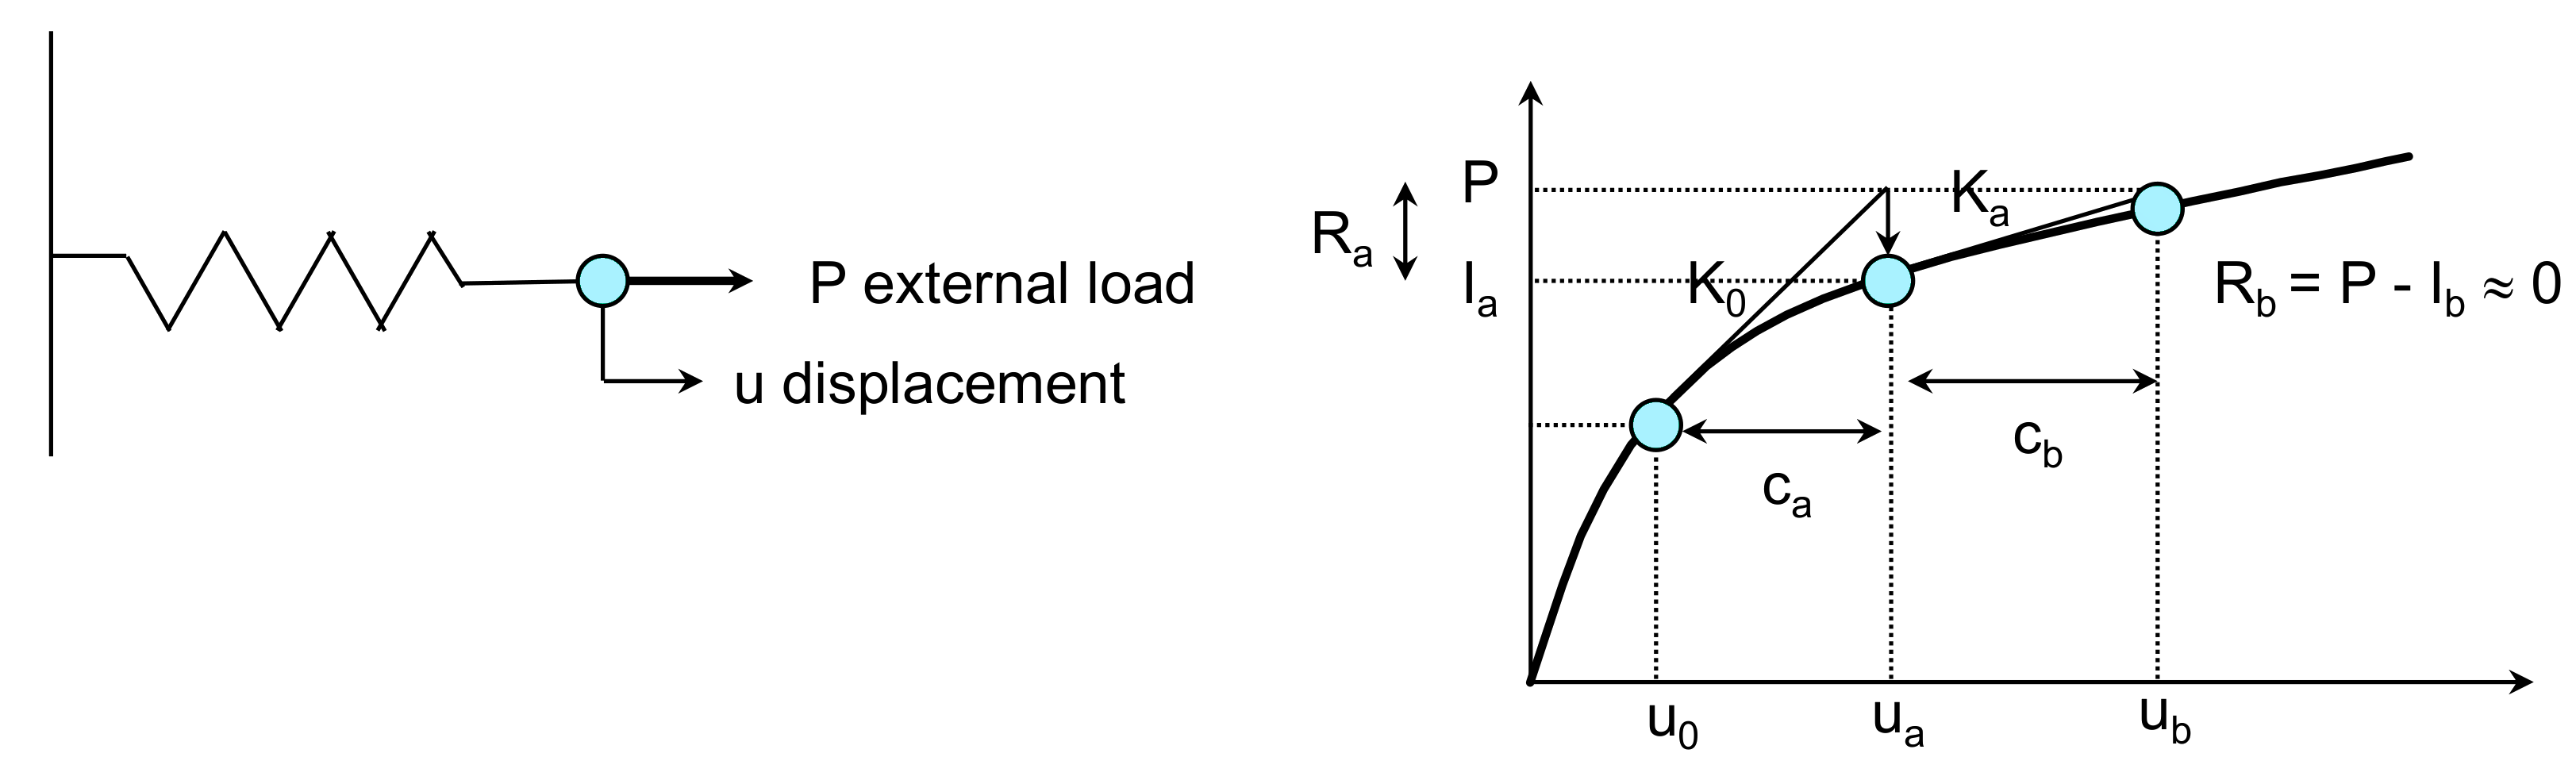
\includegraphics[width=\textwidth]{figs/newton-raphson.png}
	\end{figure}
	\begin{itemize}
		\item Using the initial stiffness $K_0$, apply an increment of load $\delta P$,
		calculate an approximate solution $c_a$ caused by this increment.
		
		\item The stiffness $K_a$ is updated using the new position, and the
		internal force in the spring $I_a$ is calculated.
		
		\item If the difference $R_a$ between the total load applied to the spring,
		$P$, and $I_a$ is smaller than the tolerance, $u_a = u_0 + c_a$ is the
		converged solution.
	\end{itemize}
}
\mode<handout>{
	\vspace{6cm}
}
\end{frame}

\note{
	\begin{itemize}
		\item If $R_a$ is not small, a new displacement correction $c_b$ is calculated
		by solving $c_b = R_a /K_a$
		\item The new displacement $u_b$ is updated, and the internal force $I_b$ in
		the updated configuration is calculated.
		\item The new force residual $R_b$ is obtained. If $R_b < tolerance$, the
		solution is converged. If not, continue the iteration.
	\end{itemize}
}


%------------------------------------------------
\begin{frame}
\frametitle{Newton Raphson method: Tolerance and Convergence}
\begin{itemize}
	\item Program - ABAQUS
	\item Newton-Raphson is the most standard method to solve nonlinear problems in FE.
	\item A large error in the initial estimate can contribute to non-convergence of the algorithm.
	\item \textbf{Tolerance}
	\begin{itemize}
		\item must be small enough to ensure that the approximate
		solution is close to the exact mathematical solution.
		\item must be large enough so that reasonable number of
		iterations are performed.
	\end{itemize}
	\item \textbf{Quadratic convergence}
	\begin{itemize}
		\item If the tangent stiffness is calculated correctly, $R$ should
		reduce quadratically from one iteration to the next.
	\end{itemize}
\end{itemize}
\end{frame}
\end{document}